\documentclass[11pt]{article}

\usepackage[margin=1in]{geometry}
\usepackage{caption}
\usepackage{graphicx}
\usepackage[hidelinks]{hyperref}
\usepackage{microtype}
\usepackage{siunitx}

\sisetup{
  detect-all,
  scientific-notation=true,
  round-mode=places,
  round-precision=3
}

\title{Draft Methods and Results: Belief Geometry in MESS3 Agents}
\author{Author names to be added}
\date{\today}

\begin{document}
\maketitle

\section{Predicting the next MESS3 token}
\label{sec:token-guess}

\subsection{Task}

We first studied a passive three-state hidden Markov process with three emitted
symbols. The latent state persisted with probability \(0.90\) and transitioned
to either other state with probability \(0.05\). State \(i\) emitted symbol
\(i\) with probability \(0.85\), with the remaining probability split equally
between the other symbols. The agent observed only emitted symbols, not the
latent state, and selected one of three symbols as its prediction of the next
delivered emission. A correct prediction yielded reward 1 and an incorrect
prediction reward 0. Actions did not alter the process dynamics. Episodes
contained 512 steps, with the first episode length randomized to reduce
synchronization artifacts.

\subsection{Model architecture}

The token-guess agent used the small MESS3 transformer architecture of
Shai et al.~\cite{shai2024transformers}. A bias-free linear map embedded each
three-dimensional token one-hot into a 64-dimensional residual stream, to
which learned absolute position embeddings were added. The trunk contained
four pre-layer-normalized causal transformer blocks. Each block used one
attention head with 8-dimensional queries, keys, and values, followed by a
256-dimensional ReLU feed-forward sublayer; residual connections surrounded
both sublayers. The model processed a right-aligned context of 10 observations
and applied a final layer normalization to the most recent position. Linear
\(64\!\rightarrow\!3\) and \(64\!\rightarrow\!1\) heads produced categorical
policy logits and a scalar value estimate, respectively. Objective-specific
heads are described next.

\subsection{Training objectives and heads}

All three reported conditions used PPO and the same initialization for a given
model seed. Because reward was immediate prediction correctness, we set
\(\gamma=\lambda=0\). PPO used Adam with learning rate
\(10^{-4}\), clipping parameter \(0.2\), no KL penalty, value-loss coefficient
\(0.5\), no entropy bonus, batches of 32,768 agent steps, minibatches of 4,096,
and six optimization epochs per batch. Every condition had the shared
three-logit policy head and scalar value head.

\begin{itemize}
  \item \textbf{PPO} optimized only the clipped policy objective for binary
    prediction correctness and the value loss.
  \item \textbf{PPO + next-token CE} added a training-only linear
    \(64\!\rightarrow\!3\) head. Its cross-entropy against the next emitted
    symbol entered the loss with coefficient 1.
  \item \textbf{PPO + decoupled Kelly} added a separate training-only linear
    \(64\!\rightarrow\!3\) wager head. The logit corresponding to the selected
    action parameterized a sigmoid wager. Correct predictions received net
    odds \(2{:}1\), incorrect predictions lost the wager, and negative realized
    log growth entered the PPO loss with coefficient 1. This auxiliary head
    did not replace or share parameters with the categorical policy head.
\end{itemize}

The campaign used 15 paired model seeds (45--59) and a nominal budget of
700,000 agent steps. Because stopping was checked at batch boundaries, final
checkpoints occurred between 725,089 and 728,210 steps. We retained
initialization, approximately 0.33M and 0.66M steps, and the final checkpoint.
The planned paired comparison used the approximately 0.66M-step checkpoint.

\subsection{Belief probe}

At each retained checkpoint, we evaluated whether the transformer's
post-final-layer-normalization residual stream linearly encoded the exact
Bayesian belief over the three latent states. We fit an affine ridge probe
(\(10^{-6}\) penalty) on 60,000 steps and evaluated it on an independent
80,000-step rollout, distributed across 16 environments under the greedy
policy. The reported MSE is the mean squared error between the three-component
decoded and exact beliefs. Per-run 95\% intervals used 1,000 percentile
bootstrap resamples clustered by environment episode, with the fitted probe
held fixed. Figure~\ref{fig:token-mse} summarizes variation across model seeds
as the mean \(\pm\) one population standard deviation.

\subsection{Results}

At initialization, mean held-out probe MSE was
\(3.949\times10^{-3}\) (SD \(3.987\times10^{-4}\)) in all three paired
conditions. By the prespecified comparison checkpoint, mean MSE was
\(3.904\times10^{-4}\) for PPO,
\(4.236\times10^{-4}\) for PPO + next-token CE, and
\(2.833\times10^{-4}\) for PPO + decoupled Kelly. In paired comparisons by
model seed, the decoupled-Kelly condition reduced MSE relative to next-token CE
by \(1.403\times10^{-4}\)
(\(t_{14}=-5.734,\ p=5.17\times10^{-5}\)) and relative to PPO by
\(1.071\times10^{-4}\)
(\(t_{14}=-6.052,\ p=2.97\times10^{-5}\)).

At the final checkpoint, mean MSE was
\(4.083\times10^{-4}\) (SD \(6.399\times10^{-5}\)) for PPO,
\(4.111\times10^{-4}\) (SD \(1.007\times10^{-4}\)) for next-token CE, and
\(2.862\times10^{-4}\) (SD \(4.785\times10^{-5}\)) for decoupled Kelly.
Thus, all objectives produced an approximately order-of-magnitude reduction
from initialization, while the decoupled-Kelly objective remained lowest at
the end of training. This result establishes linear decodability of Bayesian
belief; it does not by itself show that the policy causally used the decoded
belief.

\begin{figure}[t]
  \centering
  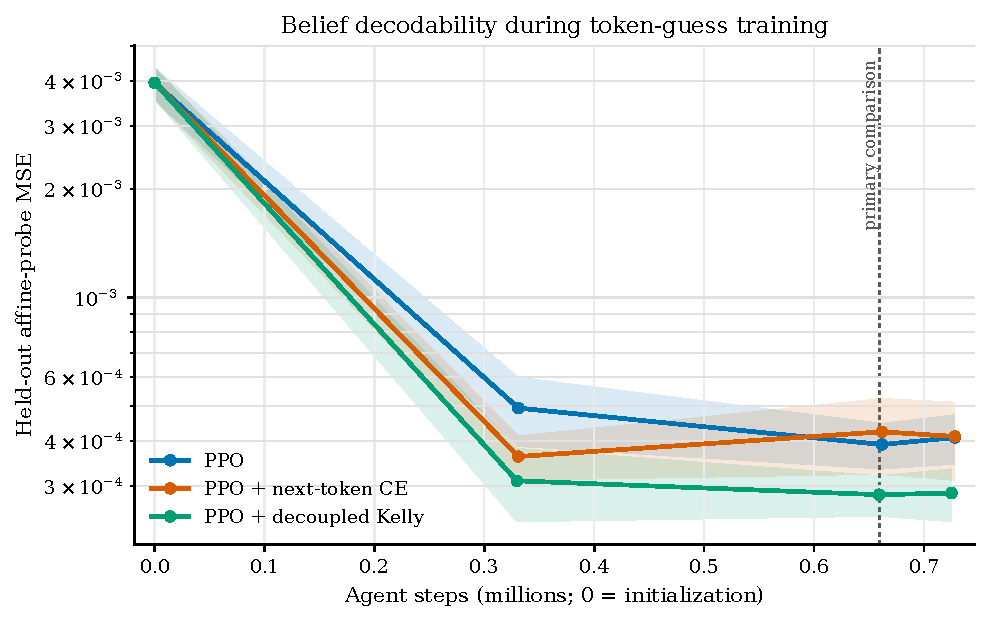
\includegraphics[width=0.94\linewidth]{figures/token_guess_cycle2_mse.pdf}
  \caption{Held-out affine-probe MSE over token-guess training. Lines show the
  mean across 15 paired model seeds and shaded regions show one population
  standard deviation. The vertical dotted line marks the checkpoint used for
  paired inference. Step zero is the untrained, seed-matched initialization.
  Lower values indicate more accurate linear decoding of the exact Bayesian
  belief from the final normalized residual stream.}
  \label{fig:token-mse}
\end{figure}

\section{Controlling occupancy of a reward state}
\label{sec:action-symmetry}

\subsection{Task}

The second study made MESS3 controllable. The agent received the current
one-hot symbol and the previous one-hot action, selected among
\emph{noop}, \emph{positive}, and \emph{negative}, and received reward 1 when
the current latent state was state 2. The emission channel again had accuracy
0.85. The uncontrolled transition rows were
\[
  (0.75,0.15,0.10),\quad
  (0.15,0.75,0.10),\quad
  (0.30,0.30,0.40).
\]
An active action changed the odds of transitioning into state 2 by a factor
\(\exp(\pm1.5)\), while preserving the relative odds of transitions into
states 0 and 1. The three variants differed only in where the sign of this
action effect was applied:
\begin{enumerate}
  \item positive increased state-2 odds from every source state;
  \item positive increased state-2 odds outside state 2 but decreased them
    inside state 2, making noop optimal when state 2 was sufficiently likely;
  \item positive and negative had symmetric roles in source states 0 and 1,
    while both decreased state-2 retention, again making noop optimal in
    state 2.
\end{enumerate}
The corresponding fully observed optimal policies were
\([\text{positive},\text{positive},\text{positive}]\),
\([\text{positive},\text{positive},\text{noop}]\), and
\([\text{positive},\text{negative},\text{noop}]\). Episodes contained 1,024
steps with randomized first-episode length.

\subsection{Model architecture}

The action-symmetry agent received a six-dimensional observation formed by
concatenating one-hot encodings of the current symbol and previous action. A
linear input projection mapped this vector into a 96-dimensional residual
stream. The trunk contained three pre-layer-normalized causal transformer
blocks, each with four 24-dimensional attention heads, rotary position
embeddings on queries and keys, and a 384-dimensional GELU feed-forward
sublayer. Attention was banded to the preceding 64 positions at each layer,
giving the three-layer stack a 192-step raw-observation receptive field. A
final layer normalization fed linear \(96\!\rightarrow\!3\) categorical-policy
and \(96\!\rightarrow\!1\) scalar-value heads.

\subsection{Training algorithm and heads}

Each variant used plain PPO with only the shared categorical policy head and
scalar value head; no auxiliary prediction or belief loss was applied. PPO
used Adam with learning rate \(4.2\times10^{-4}\),
\(\gamma=0.99\), \(\lambda=0.95\), clipping parameter \(0.2\), value-loss
coefficient \(0.5\), entropy coefficient \(0.003\), batches of 32,768
environment steps, minibatches of 2,048, and six optimization epochs. The
nominal training budget was 700,000 environment steps per variant. Probes were
scheduled at initialization, iterations 1, 2, 4, and 8, and the final
checkpoint. Belief MSE used the same held-out 60,000/80,000-step affine-probe
protocol described in Section~\ref{sec:token-guess}. Each variant was trained
with five model seeds (42--46). Batch-boundary stopping placed the final
checkpoints between 728,658 and 728,664 environment steps.

\subsection{Results}

The variants developed sharply different representational trajectories
(Figure~\ref{fig:action-symmetry-mse}). Variant 1 began at mean MSE
\(4.667\times10^{-3}\) and worsened to
\(6.038\times10^{-3}\) (SD \(4.993\times10^{-4}\)) at the final checkpoint.
Variant 2 fell from \(4.281\times10^{-3}\) at initialization to
\(2.804\times10^{-3}\) near 0.27M steps, then ended at
\(3.495\times10^{-3}\) (SD \(4.213\times10^{-4}\)). Variant 3 showed the
largest improvement, falling from \(4.970\times10^{-3}\) to
\(3.402\times10^{-4}\) near 0.27M steps before rising to
\(1.211\times10^{-3}\) (SD \(2.578\times10^{-4}\)) at the final checkpoint.
Despite this late increase, variant 3's final MSE remained 65\% below variant
2 and 80\% below variant 1.

The learned greedy policies help contextualize this ordering. Variant 1
collapsed to the positive action in all five seeds and attained reward-state
occupancy \(0.571\pm0.004\), but had the least linearly decodable beliefs.
Variant 2 consistently mixed noop and positive actions in proportions
\(0.33/0.67\), attaining occupancy \(0.331\pm0.002\). Variant 3 maintained an
approximately balanced noop/positive/negative mixture
\((0.32/0.34/0.34)\), attained occupancy \(0.314\pm0.002\), and had the lowest
probe MSE. These results show that maximizing reward-state occupancy and
preserving an affinely decodable Bayesian belief were not aligned across the
three control symmetries. As above, the probe establishes decodability rather
than causal policy use.

\begin{figure}[t]
  \centering
  \includegraphics[width=0.94\linewidth]%
    {figures/action_symmetry_cycle4_mse.pdf}
  \caption{Held-out affine-probe MSE over action-symmetry training. Lines show
  means across five model seeds and shaded regions show one population
  standard deviation. Step zero is the untrained initialization. Variant 3
  reached its minimum mean MSE near 0.27M steps, whereas variant 1's MSE
  increased over training.}
  \label{fig:action-symmetry-mse}
\end{figure}

\begin{thebibliography}{1}
\bibitem{shai2024transformers}
Adam S. Shai, Sarah E. Marzen, Lucas Teixeira, Alexander Gietelink Oldenziel,
and Paul M. Riechers.
\newblock Transformers represent belief state geometry in their residual
stream.
\newblock In \emph{Advances in Neural Information Processing Systems}, 2024.
\end{thebibliography}

\end{document}
